% !TeX root = orbits.tex

%%%%%%%%%%%%%%%%%%%%%%%%%%%%%%%%%%%%%%%%%%%%%%%%%%%%%%%%%%%%%%%%

\section{Gravitation}\label{s.newton}

In this section we present Isaac Newton's demonstrations that the inverse-square law can be deduced from Kepler's observation that the orbits of planets are ellipses. After a review of Newton's Laws of force and motion,  we show that Kepler's second law must hold in any system subject to a centripetal force. The next step is to show that the inverse square law for gravitation must hold in an elliptical orbit. Then it is a small step to universal gravitation and Kepler's third law. For readers who wish to study the \emph{Principia} the labels of the points in the diagrams are the same as those used by Newton.

\subsection{Newton's laws of motion}

\begin{enumerate}
\item A body in uniform motion (including a body at rest) continues with the same motion unless a force is applied.
\item A force $F$ applied to a body causes an acceleration $a$ in the direction of the force whose magnitude $a=F/m$, where $m$, the constant of proportionality, is called the \emph{mass} of the body.
\item If one body exerts a force on a second body, the second body exerts a force on the first of equal magnitude but in the opposite direction.
\end{enumerate}
Forces are denoted by vectors, where the direction of the vector represents the direction of the force and the length of the vector represents the magnitude of the force. Forces can be decomposed into perpendicular components (Figure~\ref{f.grav-forces1}), or into components in any directions (Figure~\ref{f.grav-forces2}). The components form a parallelogram whose diagonal is the resultant force.

%%%%%%%%%%%%%%%%%%%%%%%%%%%%%%%%%%%%%%%%%%%%%%%%%%%%%%%%%%%%%%%%

\begin{figure}[b]
\begin{minipage}{.45\textwidth}
\begin{center}
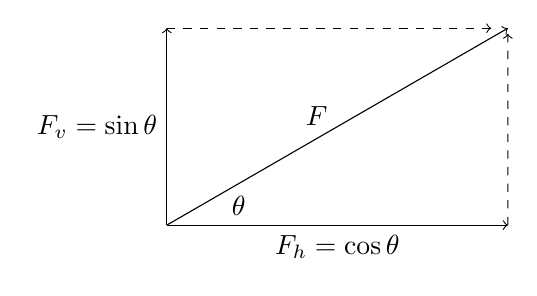
\begin{tikzpicture}

% Define center point
\coordinate (O) at (0,0);
\node[above right,xshift=20pt] at (O) {$\theta$};

% Construct force vector
\draw[->] (O) -- node[left,yshift=4pt] {$F$} +(30:5) coordinate (F);

% Construct horizontal component
\draw[->] (O) -- node[below] {$F_h=\cos \theta$} +(0:4.33) coordinate (FH);
\draw[->,style={shorten >= 2pt},dashed] (FH) -- (F);

% Construct vertical component
\draw[->] (O) -- node[left] {$F_v=\sin \theta$} +(90:2.5) coordinate (FV);
\draw[->,style={shorten >= 6pt},dashed] (FV) -- (F);
\end{tikzpicture}
\caption{Perpendicular components of a force}\label{f.grav-forces1}
\end{center}
\end{minipage}
%%%%%%%%%%%%%%
\hfill
\begin{minipage}{.45\textwidth}
\begin{center}
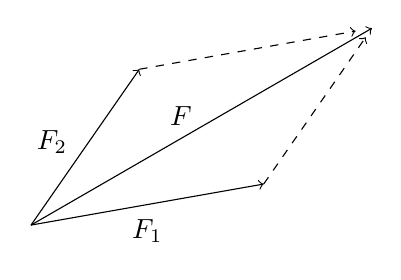
\begin{tikzpicture}

% Define center piont
\coordinate (O) at (0,0);

% Construct force vector
\draw[->] (O) -- node[left,yshift=4pt] {$F$} +(30:5) coordinate(F);

% Construct one component
\draw[->] (O) -- node[below,yshift=-2pt] {$F_1$} +(10:3) coordinate (F1);
\draw[->,style={shorten >= 4pt},dashed] (F1) -- (F);

% Construct other component
% First define end of component to allow shortened arrow
\path[dashed] (F) -- +(190:3) coordinate (F2);
\draw[->,style={shorten >= 6pt},dashed] (F2) -- (F);
\draw[->] (O) --  node[left,xshift=-3pt,yshift=2pt] {$F_2$} (F2);
\end{tikzpicture}
\caption{Arbitrary components of a force}\label{f.grav-forces2}
\end{center}
\end{minipage}
\end{figure}

%%%%%%%%%%%%%%%%%%%%%%%%%%%%%%%%%%%%%%%%%%%%%%%%%%%%%%%%%%%%%%%%

Newton was interested in \emph{centripetal force} which is a force exerted by a single body on another, in particular, the gravitational force exerted by the Sun on a planet (Figure~\ref{f.grav-centripetal}). Since the only force is that directed towards the Sun, the planet does not move ``up'' or ``down'' so its orbit is in a plane.

%%%%%%%%%%%%%%%%%%%%%%%%%%%%%%%%%%%%%%%%%%%%%%%%%%%%%%%%%%%%%%%%

\begin{figure}[tb]
\begin{minipage}{.48\textwidth}
\begin{center}
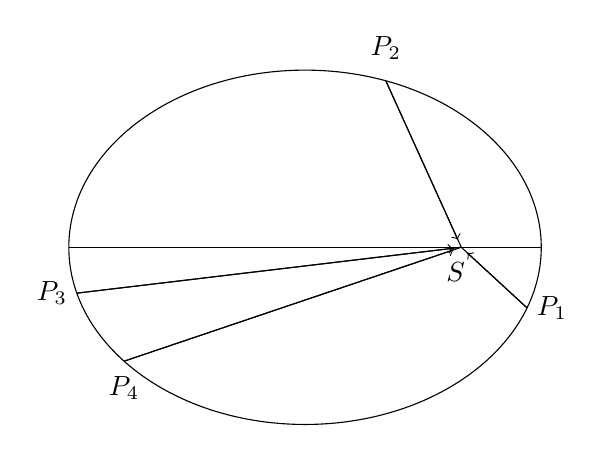
\begin{tikzpicture}[scale=.75]

% Size and center of the ellipse
\def\a{4}
\def\b{3}
\coordinate (O) at (0,0);

% Draw axis/axes through O
\coordinate (L) at (-180:{\a} and {\b});
\coordinate (R) at (0:{\a} and {\b});
\draw (L) -- (R);

% The Sun is at a focal point
\coordinate (Sun) at ({+sqrt(\a*\a-\b*\b)},0);
\node[below,xshift=-2pt,yshift=-2pt] at (Sun) {$S$};

% Locate and label four arbitrary points on the list
\coordinate (P1) at +(-20:{\a} and {\b});
\draw (P1) node[right] {$P_1$} -- (Sun);
\coordinate (P2) at +(70:{\a} and {\b});
\draw (P2) node[above,yshift=4pt] {$P_2$} -- (Sun);
\coordinate (P3) at +(195:{\a} and {\b});
\draw (P3) node[left] {$P_3$} -- (Sun);
\coordinate (P4) at +(220:{\a} and {\b});
\draw (P4) node[below,yshift=-2pt] {$P_4$} -- (Sun);

% Draw the ellipse and bullets for the points
%   over the shade
\draw (0,0) ellipse({\a} and {\b});
%\vertexsm{Sun};
%\vertexsm{P1};
%\vertexsm{P2};
%\vertexsm{P3};
%\vertexsm{P4};

% Construct the arrows
\draw[->,style={shorten >= 3pt}] (P1) -- (Sun);
\draw[->,style={shorten >= 3pt}] (P2) -- (Sun);
\draw[->,style={shorten >= 3pt}] (P3) -- (Sun);
\draw[->,style={shorten >= 3pt}] (P4) -- (Sun);

\end{tikzpicture}
\caption{Centripetal force}\label{f.grav-centripetal}
\end{center}
\end{minipage}
%%%%%%%%%%%%%%
\begin{minipage}{.5\textwidth}
\begin{center}
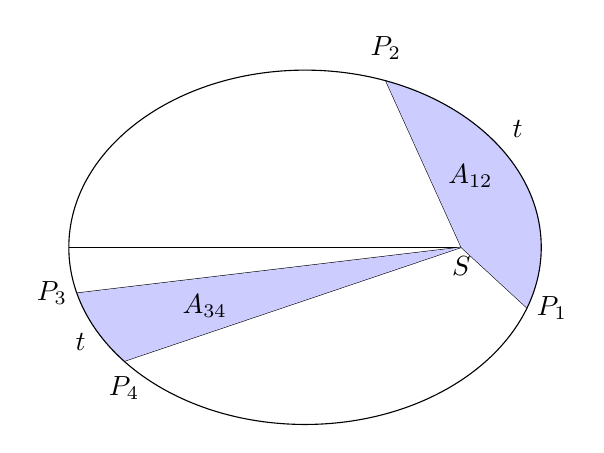
\begin{tikzpicture}[scale=.75]

% Size and center of the ellipse
\def\a{4}
\def\b{3}
\coordinate (O) at (0,0);

% Draw axis/axes through O
\coordinate (L) at (-180:{\a} and {\b});
\coordinate (R) at (0:{\a} and {\b});
\draw (L) -- (R);

% The Sun is at a focal point
\coordinate (Sun) at ({+sqrt(\a*\a-\b*\b)},0);
\node[below] at (Sun) {$S$};

% Locate and label four arbitrary points on the list
\coordinate (P1) at +(-20:{\a} and {\b});
\draw (P1) node[right] {$P_1$} -- (Sun);
\coordinate (P2) at +(70:{\a} and {\b});
\draw (P2) node[above,yshift=4pt] {$P_2$} -- (Sun);
\coordinate (P3) at +(195:{\a} and {\b});
\draw (P3) node[left] {$P_3$} -- (Sun);
\coordinate (P4) at +(220:{\a} and {\b});
\draw (P4) node[below,yshift=-2pt] {$P_4$} -- (Sun);

% Shade the sectors
\fill[blue!20] (Sun) -- (P1) arc [start angle = -20, end angle = 70,
    x radius = \a, y radius = \b] -- (P2) -- cycle;
\fill[blue!20] (Sun) -- (P3) arc [start angle = 195, end angle = 220,
    x radius = \a, y radius = \b] -- (P4) -- cycle;

% Draw the ellipse and bullets for the points
%   over the shade
\draw (0,0) ellipse({\a} and {\b});
%\vertexsm{Sun};
%\vertexsm{P1};
%\vertexsm{P2};
%\vertexsm{P3};
%\vertexsm{P4};

% Label the times and areas
\node at (3.6,2) {$t$};
\node at (-3.8,-1.6) {$t$};
\node at (2.8,1.2) {$A_{12}$};
\node at (-1.7,-1) {$A_{34}$};
\end{tikzpicture}
\caption{Equal areas in equal times}\label{f.grav-second}
\end{center}
\end{minipage}
\end{figure}

%%%%%%%%%%%%%%%%%%%%%%%%%%%%%%%%%%%%%%%%%%%%%%%%%%%%%%%%%%%%%%%%

Kepler's second law states that a planet in orbit sweeps out equal area in intervals of equal duration, if it takes the planet time $t$ to move from $P_1$ to $P_2$ and also $t$ to move from $P_3$ to $P_4$, then $A_{12}$, the area of the sector $P_1SP_2$, is equal to $A_{34}$, the area of $P_3SP_4$ (Figure~\ref{f.grav-second}). Obviously, this means that the speed of the planet must vary as it traverses its orbit $v_{P_1P_2} \gg v_{P_3P_4}$. Newton proved that this must be true in any system where a body is subject to a centripetal force from another body. 

The proof is based on dividing an area into very small sectors and then taking the limit. Consider three points $A,B,C$ on the orbit (Figure~\ref{f.grav-very-small}) that represent the positions of the planet at intervals of $\Delta t$. For clarity we have drawn them spaced out, but the intention is that they are very close together. Newton assumed that the planet does not smoothly traverse the arcs, but rather that it every $\Delta t$ it jumps in discrete steps from one point on the orbit to the next.

%%%%%%%%%%%%%%%%%%%%%%%%%%%%%%%%%%%%%%%%%%%%%%%%%%%%%%%%%%%%%%%%

Figure~\ref{f.grav-small} shows how the force is exerted in discrete steps. The planet moves from $A$ to $B$ and we expect that the centripetal force at $B$ will cause an acceleration that moves the planet to $C$, the next point on the orbit. Instead, we ``pretend'' that the force is not applied at $B$, but, in the absence of an applied force, planet continues to move in the same direction and at the same speed. After another period of $\Delta t$ as passed and the planet has reached point $C'$, the force is now applied \emph{in the same direction} as it would have been applied at $B$, moving the planet to $C$. 

\begin{figure}[tb]
\begin{minipage}{.48\textwidth}
\begin{center}
\begin{tikzpicture}[scale=1.4]

% Align captions

\path (4,4.1) -- +(1,0);

% Size and center of the ellipse
\def\a{5}
\def\b{4}
\coordinate (O) at (0,0);

% The Sun is at a focal point
\coordinate (S) at ({+sqrt(\a*\a-\b*\b)},0);
\node[below] at (S) {$S$};
%\vertexsm{S};

% Construct the ellipse
\draw[name path=ellipse] (5,0) arc(0:60:5cm and 4cm);

% Locate and label three arbitrary points on the list
\path [name path=a] (S) -- ($(S)+(10:3)$);
\path [name intersections = {of = ellipse and a, by = {A} }];
\draw (S) -- (A) node[right] {$A$};
%\vertexsm{A};
\path [name path=b] (S) -- ($(S)+(50:3)$);
\path [name intersections = {of = ellipse and b, by = {B} }];
\draw (S) -- (B) node[above right] {$B$};
%\vertexsm{B};
\path [name path=c] (S) -- ($(S)+(82:3)$);
\path [name intersections = {of = ellipse and c, by = {C} }];
\draw (S) -- (C) node[above] {$C$};
%\vertexsm{C};

% Label A, B, C
\path (A) --
  node[right,xshift=8pt,yshift=2pt] {$\Delta t$} (B) -- 
  node[above right,xshift=4pt] {$\Delta t$} (C);

\end{tikzpicture}
\caption{``Small'' sectors of an orbit}\label{f.grav-very-small}
\end{center}
\end{minipage}
%%%%%%%%%%%%%%
\begin{minipage}{.48\textwidth}
\begin{center}
\begin{tikzpicture}[scale=1.4]

% Size and center of the ellipse
\def\a{5}
\def\b{4}
\coordinate (O) at (0,0);

% The Sun is at a focal point
\coordinate (S) at ({+sqrt(\a*\a-\b*\b)},0);
\node[below] at (S) {$S$};
%\vertexsm{S};

% Construct the ellipse
\draw[name path=ellipse] (5,0) arc(0:60:5cm and 4cm);

% Locate and label four arbitrary points on the list
\coordinate (A) at +(5:{\a} and {\b});
\draw (S) -- (A) node[right] {$A$};
%\vertexsm{A};
\coordinate (B) at +(30:{\a} and {\b});
\draw (B) node[above right] {$B$} -- (S);
%\vertexsm{B};

% Draw the force arrow
\coordinate (BX) at ($(B)+(.2,0)$);
\coordinate (SX) at ($(S)+(.2,0)$);
\draw[->] ($(BX)!.3!(SX)$) -- node[right,near end,xshift=2pt] {$F_B$} ($(BX)!.6!(SX)$);

% Draw AB
\draw (A) --
  node[right,xshift=8pt,yshift=2pt] {$\Delta t$} (B);

% Locate C' twice the length AB from A
\path (A) -- ($(A) ! 2 ! (B)$) coordinate (CP);
\vertexsm{CP};
\draw[thick,dashed] (B) -- 
  node[above right] {$\Delta t$} (CP) node[above left] {$C'$};

% Draw vector in the direction of BS
%  and locate its intersection with the ellipse
% Locate Cnew as the correct location of C
\path[name path=cp] (CP) -- +(230:2);
\path [name intersections = {of = cp and ellipse, by = {Cnew} }];
%\vertexsm{Cnew};
\draw[very thick,dashed,->] (CP) -- 
  (Cnew) node[above,xshift=-2pt,yshift=2pt] {$C$};
\draw (Cnew) -- (S);

% Draw the force arrow
\path (CP) -- ($(CP)!1.5!(Cnew)$) coordinate (CX) --
  ($(CP)!2.5!(Cnew)$) coordinate (CY);
\draw[->] (CX) -- node[left,near start,xshift=-2pt] {$F_B$} (CY);

\end{tikzpicture}
\caption{Exerting force at discrete times}\label{f.grav-small}
\end{center}
\end{minipage}
\end{figure}

%%%%%%%%%%%%%%%%%%%%%%%%%%%%%%%%%%%%%%%%%%%%%%%%%%%%%%%%%%%%%%%%

\begin{theorem}
The area of $\triangle ASB$ is equal to the area of $\triangle BSC$.
\end{theorem}

%%%%%%%%%%%%%%%%%%%%%%%%%%%%%%%%%%%%%%%%%%%%%%%%%%%%%%%%%%%%%%%%

\begin{figure}[b]
\begin{minipage}{.48\textwidth}
\begin{center}
\begin{tikzpicture}[scale=1.4]

% Size and center of the ellipse
\def\a{5}
\def\b{4}
\coordinate (O) at (0,0);

% The Sun is at a focal point
\coordinate (S) at ({+sqrt(\a*\a-\b*\b)},0);
\node[below] at (S) {$S$};

% Construct the ellipse
\draw[name path=ellipse] (5,0) arc(0:60:5cm and 4cm);

% Locate and label four arbitrary points on the list
\coordinate (A) at +(5:{\a} and {\b});
\node[right] at (A) {$A$};
\coordinate (B) at +(30:{\a} and {\b});
\node[above right] at (B) {$B$};

% Draw triangle SAB
\draw[blue] (S) -- (A) -- (B);
\draw[blue] ($(S)+(2pt,0)$) -- ($(B)+(2pt,0)$);

% Locate C' twice the length AB from A
\path (A) -- ($(A) ! 2 ! (B)$) coordinate (CP);
\node[above] at (CP) {$C'$};

% Draw vector in the direction of BS
%  and locate its intersection with the ellipse
% Locate Cnew as the correct location of C
\path[name path=cp] (CP) -- +(230:2);
\path [name intersections = {of = cp and ellipse, by = {Cnew} }];
\draw[red] (B) -- (CP) -- (S) -- cycle;
\node[above,xshift=-2pt,yshift=2pt] at (Cnew) {$C$};
\draw (S) -- (Cnew);

% Draw altitude to ABC'
\coordinate (H) at ($(A)!(S)!(CP)$);
\node[right,xshift=6pt,yshift=2pt] at (H) {$H$};
\draw[thick,dashed,red] (H) -- (S);
\draw[thick,dashed,blue] ($(H)+(1pt,-1pt)$) -- ($(S)+(1pt,-1pt)$);
\draw[rotate=115] (H) rectangle +(4pt,4pt);

% Place dots are vertices
%\vertexsm{S};
%\vertexsm{A};
%\vertexsm{B};
\vertexsm{CP};
%\vertexsm{Cnew};
%\vertexsm{H};

\end{tikzpicture}
\caption{$\triangle ASB=\triangle BSC'$}\label{f.grav-areas1}
\end{center}
\end{minipage}
%%%%%%%%%%%
\begin{minipage}{.48\textwidth}
\begin{center}
\begin{tikzpicture}[scale=1.3]

% Align captions

\path (4,4.4) -- +(1,0);

% Size and center of the ellipse
\def\a{5}
\def\b{4}
\coordinate (O) at (0,0);

% The Sun is at a focal point
\coordinate (S) at ({+sqrt(\a*\a-\b*\b)},0);
\node[below] at (S) {$S$};

% Construct the ellipse
\draw[name path=ellipse] (5,0) arc(0:60:5cm and 4cm);

% Locate and label four arbitrary points on the list
\coordinate (A) at +(5:{\a} and {\b});
\coordinate (B) at +(30:{\a} and {\b});
\node[below,yshift=-4pt] at (B) {$B$};

% Locate C' twice the length AB from A
\path (A) -- ($(A) ! 2 ! (B)$) coordinate (CP);
\node[above,xshift=-4pt] at (CP) {$C'$};

% Draw vector in the direction of BS
%  and locate its intersection with the ellipse
% Locate Cnew as the correct location of C
\path[name path=cp] (CP) -- +(230:2);
\path [name intersections = {of = cp and ellipse, by = {Cnew} }];
\draw[red] (B) -- (CP) -- (S);
\draw[red] ($(S)+(2pt,0)$) -- ($(B)+(2pt,0)$);
\node[above,xshift=-2pt,yshift=2pt] at (Cnew) {$C$};

% Draw triangle SCB
\draw[blue] (S) -- (Cnew) -- (B) -- cycle;

% Draw parallels CC', SB
\draw[thick,dashed] ($(Cnew)!-2cm!(CP)$) -- ($(Cnew)!1.3cm!(CP)$);
\draw[thick,dashed] (B) -- ($(S)!4.3cm!(B)$);

% Draw dashed line H1C
\coordinate (H1) at ($(S)!(Cnew)!(B)$);
\node[right,yshift=-2pt] at (H1) {$H_1$};
\draw[thick,dashed,blue] (H1) -- (Cnew);
\draw[rotate=140] (H1) rectangle +(4pt,4pt);

% Draw dashed line H2C
\coordinate (H2) at ($(S)!(CP)!(B)$);
\node[right,yshift=-2pt] at (H2) {$H_2$};
\draw[thick,dashed,red] (H2) -- (CP);
\draw[rotate=140] (H2) rectangle +(4pt,4pt);

% Dots are vertices
%\vertexsm{S};
%\vertexsm{B};
%\vertexsm{CP};
%\vertexsm{Cnew};
%\vertexsm{H1};
%\vertexsm{H2};

\end{tikzpicture}
\caption{$\triangle BSC'=\triangle BSC$}\label{f.grav-areas2}
\end{center}
\end{minipage}
\end{figure}

%%%%%%%%%%%%%%%%%%%%%%%%%%%%%%%%%%%%%%%%%%%%%%%%%%%%%%%%%%%%%%%%

\begin{proof}
This will be done in two steps by showing that $\triangle ASB=\triangle BSC'$ and $\triangle BSC'=\triangle BSC$. In Figure~\ref{f.grav-areas1}, $\triangle ASB$ is shown in blue and $\triangle BSC'$ is shown in red. It is assumed that $AB=BC'$ (the planet moves from $B$ to $C'$ during the same interval $\Delta t$), so since $SH$ is the height of both triangles, their areas are equal. In Figure~\ref{f.grav-areas2}, $\triangle BSC$ is shown in blue and $\triangle BSC'$ is shown in red. It is assumed $CC'$ is parallel to $SB$ (the planet is subject to the centripetal force at $C'$ in the \emph{same} direction as the force at $B$, so the heights of both triangles to the common side $SB$ are equal and their areas are equal. It follows that $\triangle ASB=\triangle BSC'=\triangle BSC$, which we denote by $\Delta A$.\hqed
\end{proof}

\pagebreak[4]

We assume that the sectors of the orbit are each divided up into small sectors of uniform duration $\Delta t$. By the theorem, each sector has the same area $\Delta A$. Therefore, 
\[
\frac{A_{12}}{\Delta A} =\frac{t}{\Delta t} = \frac{A_{34}}{\Delta A}\,,
\]
from which Kepler's second law follows:
\begin{eqn}
\frac{A_{12}}{t} &=& \frac{A_{34}}{t}\\[4pt]
A_{12} &=& A_{34}\,.
\end{eqn}

The proof used two approximations:
\begin{itemize}
\item $\Delta A$ is an approximation of the area of each sector.
\item The force at $C'$ is an approximation to the force at $B$.
\end{itemize}
In the limit as the size of the sectors decreases, the errors become negligible.

\begin{definition}\label{def.kappa}
For a given elliptical orbit, $\kappa=\displaystyle\frac{A}{t}$, where $A$ is the area of the ellipse and $t$ is the period of the orbit, is called \emph{Kepler's constant}.
\end{definition}

%%%%%%%%%%%%%%%%%%%%%%%%%%%%%%%%%%%%%%%%%%%%%%%%

\subsection{The inverse square law for gravitation}

Newton's next step was to show that if the orbit of a planet is elliptical, the centripetal force must be proportional to the mass of the planet and inversely proportional to the square of its distance from the Sun. In Figure~\ref{f.grav-inverse1}, $S$ is the Sun, and $P$ and $Q$ are points on the orbit that are very close to each other. $PR$ is a tangent to the ellipse at $P$ and $R$ is a point such that $QR$ is parallel to $SP$.  $QT$ is constructed perpendicular to $SP$. Denote the lengths $r_P=SP$, $h=QT$, $q=QR$ and the time interval from $P$ to $Q$ by $\Delta t$.

\begin{figure}[b]
\begin{center}
\begin{tikzpicture}[scale=1.1]

% Size and center of the ellipse
\def\a{4.5}
\def\b{3}
\coordinate (O) at (0,0);

% Draw half of the ellipse
%\draw[name path=ellipse] (0,0) ellipse[x radius=\a,y radius=\b];
\draw[name path=ellipse] ({\a},0) 
  arc[start angle=0,end angle=180,x radius={\a}, y radius={\b}];

% The Sun is at a focal point
\coordinate (F1) at ({-sqrt(\a*\a-\b*\b)},0);
\coordinate (F2) at ({+sqrt(\a*\a-\b*\b)},0);
\node[below] at (F1) {$S$};
%\vertexsm{F1};

% Draw axes whose center is O
\coordinate (L) at +(180:{\a} and {\b});
\coordinate (R) at +(0:{\a} and {\b});
\coordinate (Top) at +(90:{\a} and {\b});
\draw[name path=major] (L) -- (R);
\draw[name path=minor] (O) -- (Top);

% Select an arbitrary point P on the ellipse and draw a line to the Sun
\path[name path=fromF1p] (F1) -- +(5:8);
\path [name intersections = {of = ellipse and fromF1p, by = {P} }];
\draw (F1) -- node[below,xshift=32pt,yshift=3pt] {$r_p$} (P);
%\vertexsm{P};
\node[right] at (P) {$P$};

% Select an arbitrary point Q on the ellipse and draw a line to the Sun
\path[name path=fromF1q] (F1) -- +(20:8);
\path [name intersections = {of = ellipse and fromF1q, by = {Q} }];
\draw (F1) -- (Q);
%\vertexsm{Q};
\node[above] at (Q) {$Q$};

% Draw PQ
\draw[thick,dashed] (P) -- (Q);

% Draw tangent at P
\path (F1) -- ($(F1)!1.1!(P)$);
\tkzDefLine[bisector out](F1,P,F2) \tkzGetPoint{Tan}
\draw[name path=t] ($(Tan)!.9!(P)$) -- ($(Tan)!1.35!(P)$);

% Draw QR
\path[name path=qr] (Q) -- +(10:2);
\path [name intersections = {of = t and qr, by = {R} }];
%\vertexsm{R};
\node[above right] at (R) {$R$};
\draw (Q) -- node[above] {$q$} (R);

% Draw QX
\path[name path=qx] (Q) -- +($(P)-(R)$);
\path [name intersections = {of = qx and fromF1p, by = {X} }];
\draw (Q) -- (X);

% Draw the force arrows
\coordinate (PX) at ($(P)+(0,-11pt)$);
\coordinate (SX) at ($(F1)+(0,-11pt)$);
\draw[->] ($(PX)!.01!(SX)$) --
  node[below,yshift=-6pt] {$F_P$} ($(PX)!.16!(SX)$);

% Draw force arrow from Q
\path (R) -- ($(R)!1.7!(Q)$) coordinate (RX) --
  ($(R)!3!(Q)$) coordinate (RY);
\draw[->] (RX) -- node[above] {$F_P$} (RY);

% Draw force arrow from P
\draw (Q) -- node[left] {$h$} ($(F1)!(Q)!(P)$) coordinate (T);
\node[below] at (T) {$T$};
%\vertexsm{T};

\end{tikzpicture}
\caption{The derivation of the inverse square law}\label{f.grav-inverse1}
\end{center}
\end{figure}

When a point is subject to an acceleration $a$ for a period of $\Delta t$, its displacement is $\frac{1}{2} a (\Delta t)^2$. From Newton's second law we know that at point $R$, the planet is subjected to an acceleration of $F_P/m$, so
\begin{eqn}
q &=& \frac{1}{2}\frac{F_P}{m} (\Delta t)^2\\[10pt]
F_P &=& \frac{2mq}{(\Delta t)^2}\,.
\end{eqn}

Now we compute the area of $\Delta A = \triangle SPQ = (1/2)hr_p$ and use Kepler's constant:
\begin{eqn}
\Delta t &=& \frac{\Delta A}{\kappa}=\frac{hr_P}{2\kappa}\\[6pt]
F_P &=& 2mq\cdot\frac{4\kappa^2}{(hr_P)^2}= 8\kappa^2m\cdot\frac{q}{h^2}\cdot \frac{1}{r_P^2}\,.
\end{eqn}
To obtain an inverse-square law for the force, the first two factors have to be independent of the distance. For a given planet $m$ is constant and for a given elliptical orbit $\kappa$ is constant, so the first factor does not depend on the distance. What about the second factor $q/h^2$, in particular, what value does it have if $\Delta t$ approaches zero?
\begin{theorem}\label{thm.lr-limit}
In an elliptical orbit
\[
\lim_{\Delta t \rightarrow 0} \frac{q}{h^2} = \frac{1}{L}\,,
\]
where $L$ is the length of the latus rectum of the ellipse (Definition~\ref{def.ellipse-lr}).
\end{theorem}
Newton's proof is very long and is presented separately in Section~\ref{s.centripetal}.

Since $L$ is constant for any given ellipse, the inverse square law can be written
\[
F_P = \frac{8\kappa^2m}{L}\cdot\frac{1}{r_P^2}\,.\label{eqn.inverse}
\]

\paragraph{A simplified formula for the force}

The formula can be re-written so that the constant values appearing are more familiar: $a$, the semi-major axis and $T$, the period of the orbit. By Theorem~\ref{thm.ellipse-lr}, $L\!\!=\!\!2b^2/a$ and by Theorem~\ref{thm.ellipse-area}, $\kappa = A_{\textit{\scriptsize ellipse}}/T\!\!=\!\!\pi ab/T$, so
\begin{equation}
F_P = \frac{8\kappa^2 m}{L}\cdot\frac{1}{r_P^2}
=\frac{8(\pi a b)^2 m}{T^2}\cdot \frac{a}{2b^2}\cdot\frac{1}{r_P^2}
=\frac{4\pi^2 a^3 m}{T^2}\cdot\frac{1}{r_P^2}\,.\label{eqn.planet-force}
%F_P = \frac{8\kappa^2 am}{2b^2}\cdot\frac{1}{r_P^2}
%=\frac{4\pi^2 a^2 b^2 am}{b^2 T^2}\cdot \frac{1}{r_P^2}
%=\frac{4\pi^2 a^3 m}{T^2}\cdot\frac{1}{r_P^2}\,.\label{eqn.planet-force}
\end{equation}

\paragraph{Applicability of the inverse square law}
Newton was able to show that
\begin{itemize}
\item The inverse square law applies to all conic sections including a parabola and a hyperbola, not just to an ellipse and, of course, a circle. Some comets have hyperbolic orbits and orbit the Sun only once.
\item The converse holds: if a planet is subject to an inverse-square centripetal force then the orbit must be an ellipse (or other conic section).
\item The proof assumes that a planet is a very small point, but the result holds even for large planets as long as the density of the planet is radially symmetric, that is, for a given distance from the center the density is constant.
\end{itemize}

%%%%%%%%%%%%%%%%%%%%%%%%%%%%%%%%%%%%%%%%%%%%%%%%

\subsection{Universal gravitation}

Recall Newton's third law: If one body exerts a force on a second body, the second body exerts a force on the first that is equal in magnitude but in the opposite direction. Therefore, we can equate the force that the Sun $S$ exerts on a planet $S$ with the force that the planet exerts on the Sun. Let $m$ be the mass of the planet and $M$ be the mass of the Sun. Let $F_{S\leftarrow E}$ be the forced exerted by the Sun on the Earth and let $F_{E\leftarrow S}$ be the force exerted by the Earth on the Sun. Using Equation~\ref{eqn.planet-force},
\begin{eqn}
F_{S\leftarrow E} &=& \frac{8\kappa_E^2m}{L_E}\cdot\frac{1}{r^2}=\frac{C_Em}{r^2}\\[6pt]
F_{E\leftarrow S} &=& \frac{8\kappa_S^2M}{L_S}\cdot\frac{1}{r^2}=\frac{C_SM}{r^2}\\[6pt]
\frac{C_E}{M}\cdot\frac{1}{r^2}&=&\frac{C_S}{m}\cdot\frac{1}{r^2}\,,
\end{eqn}
from some constants $C_E,C_S$.

Why are the constants different? The Earth and the Sun both rotate around their center of mass called the \emph{barycenter}, which is very close to the center of the Sun since the Sun is so much more massive than the Earth. The ellipse of the Sun's orbit is very small relative to the Earth so $A$ and $L$ are smaller, and the Sun's period is large so $T$ is larger. The different values for $8\kappa^2/L$ are encapsulated into the constants $C_E,C_S$. Let $G=\displaystyle\frac{C_E}{M}=\frac{C_S}{m}$ so that
\begin{equation}
F_{S\leftarrow E}=F_{E\leftarrow S}=G\frac{mM}{r^2}\,.\label{eqn.universal}
\end{equation}
This is Newton's law of universal gravitation. It is not specific to planetary orbits but holds between any two bodies with masses $m,M$.

\subsection{Kepler's third law}

Newton proved that Kepler's third law follows from the law of universal gravitation.
\begin{theorem}[Kepler's third law]
Let $P_1, P_2$ be two planets whose elliptical orbits have semi-major axes $a_1, a_2$ and whose orbital periods around the Sun are $T_1$ and $T_2$. Then
\[
\frac{a_1^3}{T_1^2}=\frac{a_2^3}{T_2^2}\,.
\]
\end{theorem}
\begin{proof}
By Equations~\ref{eqn.planet-force} and~\ref{eqn.universal},
\[
F=\frac{4\pi^2 a_i^3 m}{T_i^2}\frac{1}{r_i^2}=\frac{GmM}{r_i^2}\,.
\]
After canceling $m$ and $r_i$ we get
\[
\frac{a_i^3}{T_i^2}=\frac{GM}{4\pi^2}\,.
\]
$\displaystyle\frac{GM}{4\pi^2}$ is a constant that depends only on the mass of the Sun and the gravitational constant, so $\displaystyle\frac{a_i^3}{T_i^2}$ is constant for all planets rotating around the Sun.\hqed
\end{proof}
